\section{Analysis}
First we will characterize some events by their signature. Unfortunately, this is not sufficient to classify all events
properly from each other, so in the next part we will conduct a serious analysis of the spatial distribution with respect to
the variables measured by the detector. 
\subsection{Signatures of detected particles: Descriptive treatment}
On the next pages figures~\ref{fig:ee},~\ref{fig:mm},~\ref{fig:tt} and~\ref{fig:qq} show
a typical event each of the respective particle. We will not use these figures any
further, but they will give an impression how typical events look like.
The red curves indicate the data of the tracking detector, visualizing the trajectories
in the inner area. Pink squares indicate where the electron calorimeter measured energies
(which we will denote as $E_{\mathrm{ecal}}$)
with the blue squares showing their momentum. Green squares indicate the energy of the
hadron calorimeter (which we will denote as $E_{\mathrm{hcal}}$).

\begin{figure}[htpb]
    \centering
    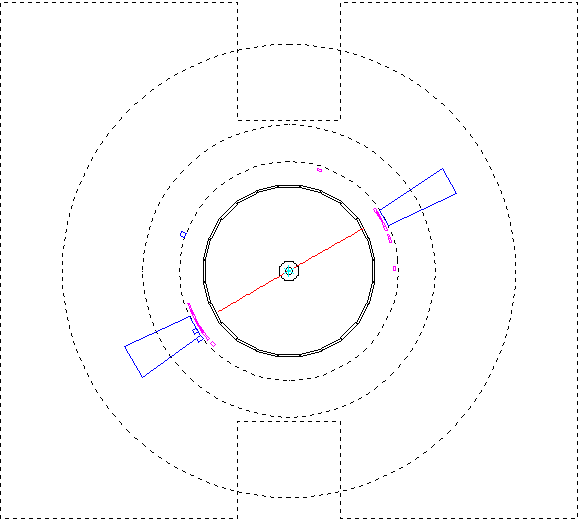
\includegraphics[width=0.8\linewidth]{figures/ee_02.png}
    \caption{Example for typical event of a decay into electrons. The characteristic feature of the decay into electrons is
    the very little number of trajectories and most of the energy submitted to first calorimeter (in the inner circle).}
\label{fig:ee}
\end{figure}

\begin{figure}[htpb]
    \centering
    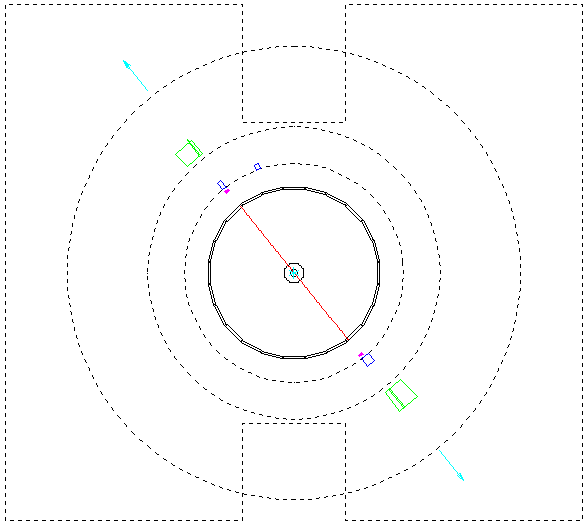
\includegraphics[width=0.8\linewidth]{figures/mm_02.png}
    \caption{Example for typical event of a decay into muons. As muons cannot be bound by the detector most of the time,
        a little amount of energy is absorbed by the first calorimeter. The muon detector far outside of this pictures (which
    is indicated by the turquoise arrows). }
\label{fig:mm}
\end{figure}

\begin{figure}[htpb]
    \centering
    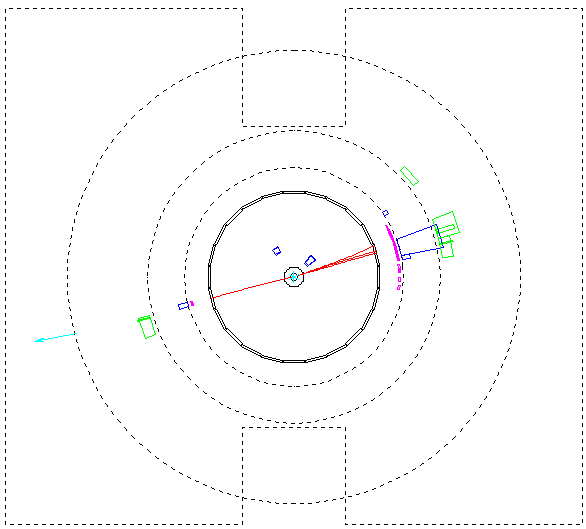
\includegraphics[width=0.8\linewidth]{figures/tt_02.png}
    \caption{Example for typical event of a decay into tauons. As the particles are not
        stopped in the first calorimeter, the probability of being electrons decreases
        significantly (this is not totally true as we will see later). Furthermore,
        there is one particle escaping to the muon detector, but not two in opposite
        directions, as we would expect for muons. There are also no hadron showers
        as characteristic for the quark branch. Hence we conclude this to be a taon event. }
\label{fig:tt}
\end{figure}

\begin{figure}[htpb]
    \centering
    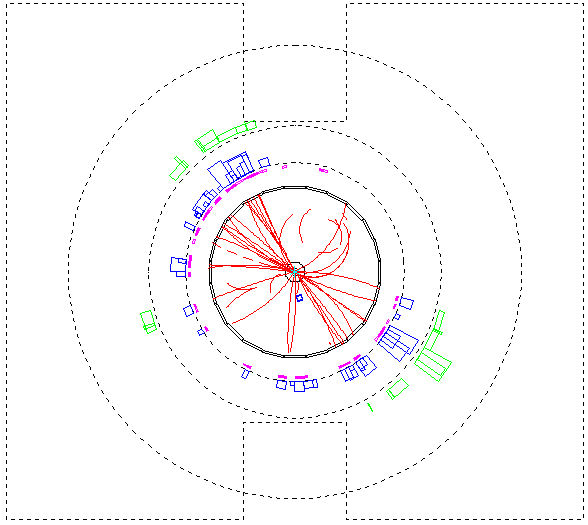
\includegraphics[width=0.8\linewidth]{figures/qq_02.png}
    \caption{Example for typical event of a decay into hadrons. As indicated in figure~\ref{fig:tt} hadronic shower are 
   a signature for quarks, originating from the \textbf{strong confinement}. 
   As bound states of quarks can only be found at low enough
   momentum, we observe a large creation of hadronic particles being
   measured in both of the calorimeter. More than half of
   the energy carried by incident hadrons is passed to additional secondaries. }
\label{fig:qq}
\end{figure}
%TODO
1. More particles, such as photon
2. Experimental setup precise 
we will do that later.


\clearpage
\subsection{Techniques used for the evaluation}
All calculations in this section are done with scripts written in 
the \textit{python} programming language~\cite{python}, relaying in several 
packages:
\begin{itemize}
    \item
        \textit{matplotlib}~\cite{Hunter2007} for plotting,
    \item
        \textit{scipy}~\cite{scipy} for fitting, and 
    \item
        \textit{uncertainties}~\cite{uc} for error propagation.
\end{itemize}
The latter applies gaussian error propagation for correlated and uncorrelated variables. 
We will thus not explicitly write down the formulas for the error propagation 
for each quantity calculated but instead state the numerical result, only. 
We will, however make a quick remark on the use of covariance matrices in 
error propagation: Contrary to measured data, which in our case is usually 
expected to be uncorrelated, all fitted data yields variables that in general correlate. 
The propagation is then done as follows:
Let's assume we have random
variables $x_0,...,x_N$ which are correlated through the $N\times N$ Matrix $cov(x_i,x_j)$.
For a scalar function $f(x_0,...,x_N) \rightarrow \mathbb{R}$, the variance is estimated (linearly) by:
\begin{equation}
Var[f] = \sigma^2 = \sum_{i,j} \frac{\partial f}{\partial x_i} \frac{\partial f}{\partial x_j} cov(x_i,x_j) \,.
\end{equation} 
If instead, $\mathbf{f}$ is a vector field in $m$ dimensions, namely 
$\mathbf{f}(x_0,...,x_N) \rightarrow \mathbb{R}^m$, then the components of $\mathbf{f}$ 
are further correlated. We can write down the relation between the covariance matrices $V$ and $U$ of 
$\mathbf{x}$ and $\mathbf{f}$, respectively, in matrix relations:
\begin{equation}
    U = A V A^T
\end{equation}
where $A$ is the matrix defined by 
\begin{equation}
    A_{ij} = \left[ \frac{\partial f_i}{\partial x_j}\right]_{\mathbf{x} = \mu}
\end{equation}
with expectation value $E[\mathbf{x}] = \mu$.~\cite{cowan1998statistical}
In order to facilitate notation, the covariance matrices will in general be notated without 
specifying the units. If not specified explicitly, the units will correspond to those of the
variables: If $x_i, x_j$ have the units $[x_i], [x_j]$, respectively, 
then the entry of the covariance matrix has the unit $[x_i] \cdot [x_j]$. 


\newpage
\section{Machine learning for classification}
As it is shown in section~\ref{sub:montecarlo} on page \pageref{sub:montecarlo} 
the different distributions of the respective particles intersect in terms of different
variables. As you might guess, the task to differentiate between particle types in the 
data is a highly non-trivial task. Therefore we searched for various techniques in order
to improve the classification of the particle species. 
As mentioned before, the analysis is done within the python
ecosystem. In particular, for the machine learning algorithms we use the library 
\textbf{scikit-learn}~\cite{scikit-learn}. 
The technique which we will present
here is used for our evaluation and turned out to be the best solution for our problem.
It is a machine learning technique called \textbf{k-nearest neighbors algorithm} and
is widely used in pattern recognition, because it is a non-parametric\footnote{
We rely on non-parametric statistics because we do not know the distributions governing
the probability of the variables of the particle species. 
The main difference in the method is that for a parametric model
the number of parameters is fixed, while in non-parametric techniques this number is 
neither fixed nor independent of the training data. This is often successful when the boundary is 
more of an irregular type.
}method which can
be implemented easily. We will not go into the implementation of the algorithm with respect to our physical problem at this
place, please refer to the appendix.
\begin{SCfigure}
    \centering
    \caption{The \textbf{k-nearest neighbors algorithm} works as following: 
        The algorithm stores all instances of the training data and their respective
    classification \textit{(colored bubbles)}. When classifying a new instance \textit{(bubble with question mark)}, the 
    predictor counts how many nearest neighbors of the unknown instance are of a specific type, the point is assigned, 
    depending on the parameter \textbf{k}, the class of the majority. In the beginning, when only the learning set is available,
    the parameter \textbf{k} is chosen such that the error of second order is minimized. In general, a larger \textbf{k} will
    limit the effects of stochastic noise but this will make the classification boundaries fuzzier.}
    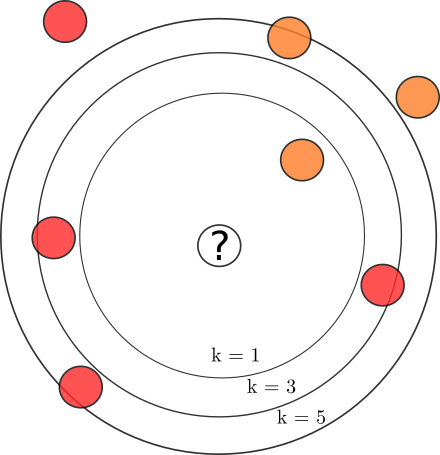
\includegraphics[width=0.5\linewidth]{figures/knn_schema}
\label{fig:knn_schema}
\end{SCfigure}

\begin{figure}[htpb]
    \centering
    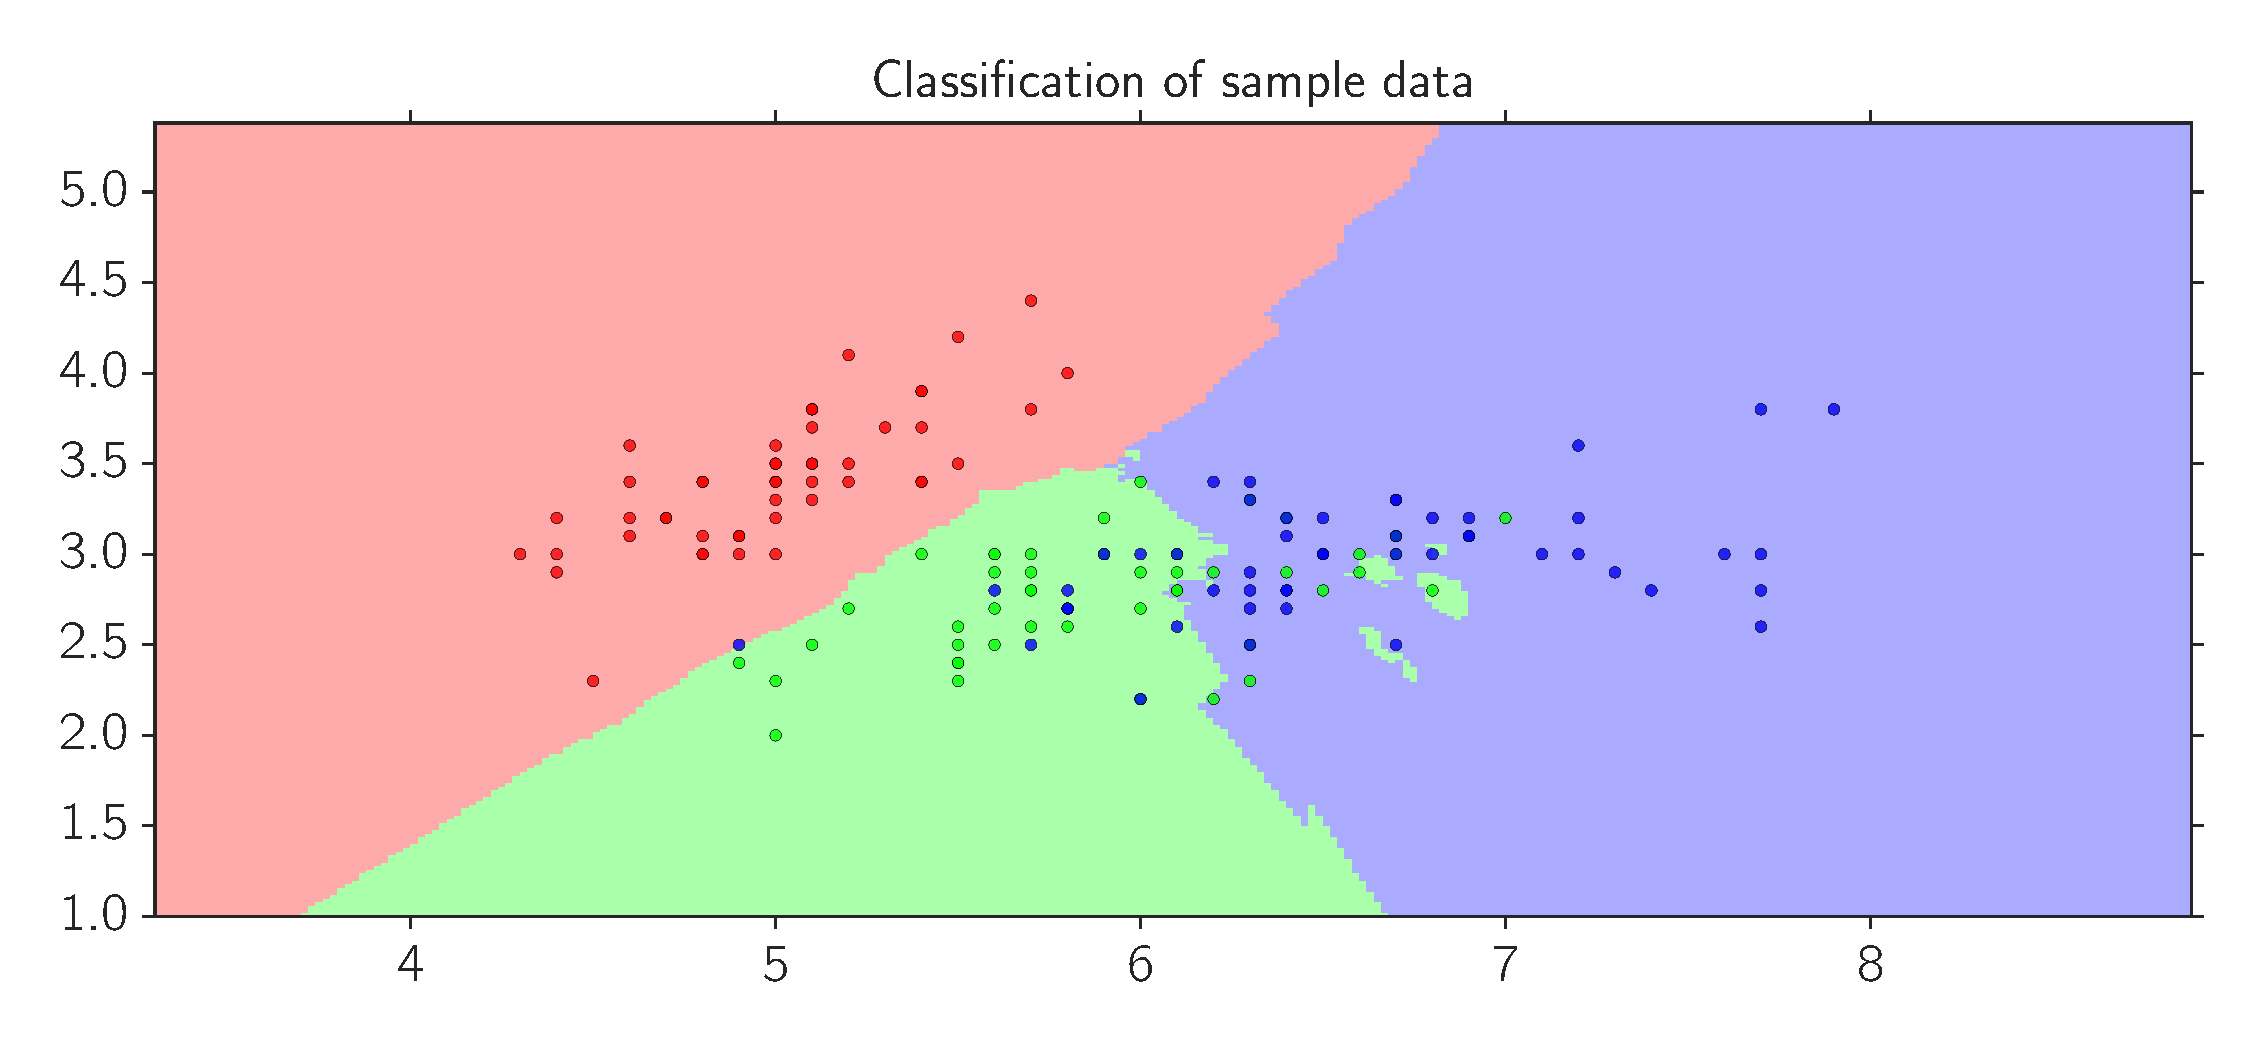
\includegraphics[width=1\linewidth]{figures/kneigbors}
    \caption{Example taken from documentary of \textbf{scikit-learn}\cite{scikit-learn}, the library we are using. Here you can
    see plotted the learning data \textit{colored dots} and the prediction for homogeneous distributed test data
(\textit{colored surface}). The data is the commonly taken \textit{Iris flower data set} \cite{frank1968numerical}, which
    is often used in order to benchmark a supervised learning algorithm. For a detailed examples of \textbf{scikit learn}
    refer to \cite{masteringscikit}.}
\label{fig:kneigbors}
\end{figure}

\subsection{Monte Carlo data}
\label{sub:montecarlo}

\begin{figure}[htpb]
    \centering
    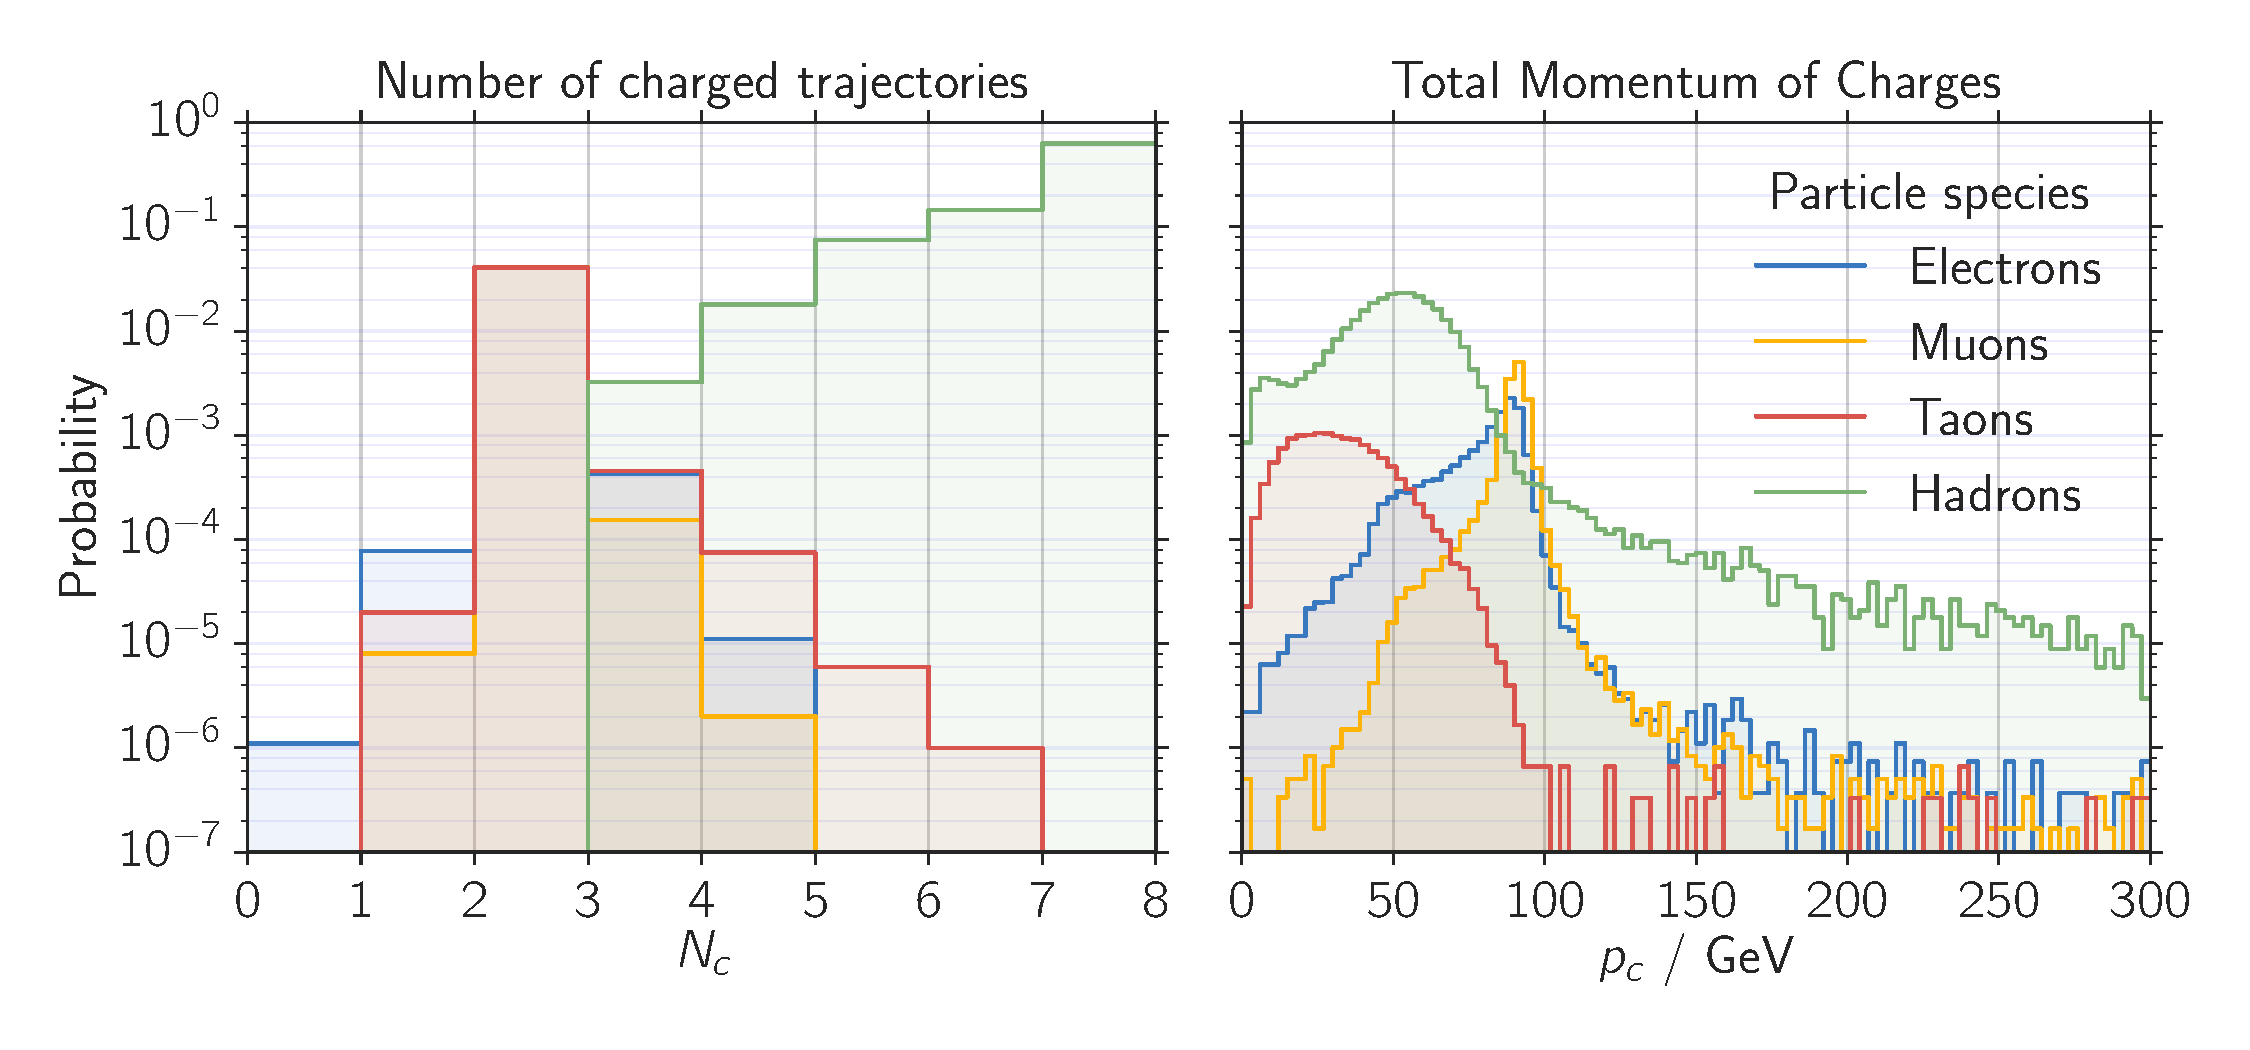
\includegraphics[width=1.0\linewidth]{figures/N_p_c}
    \caption{bla}
    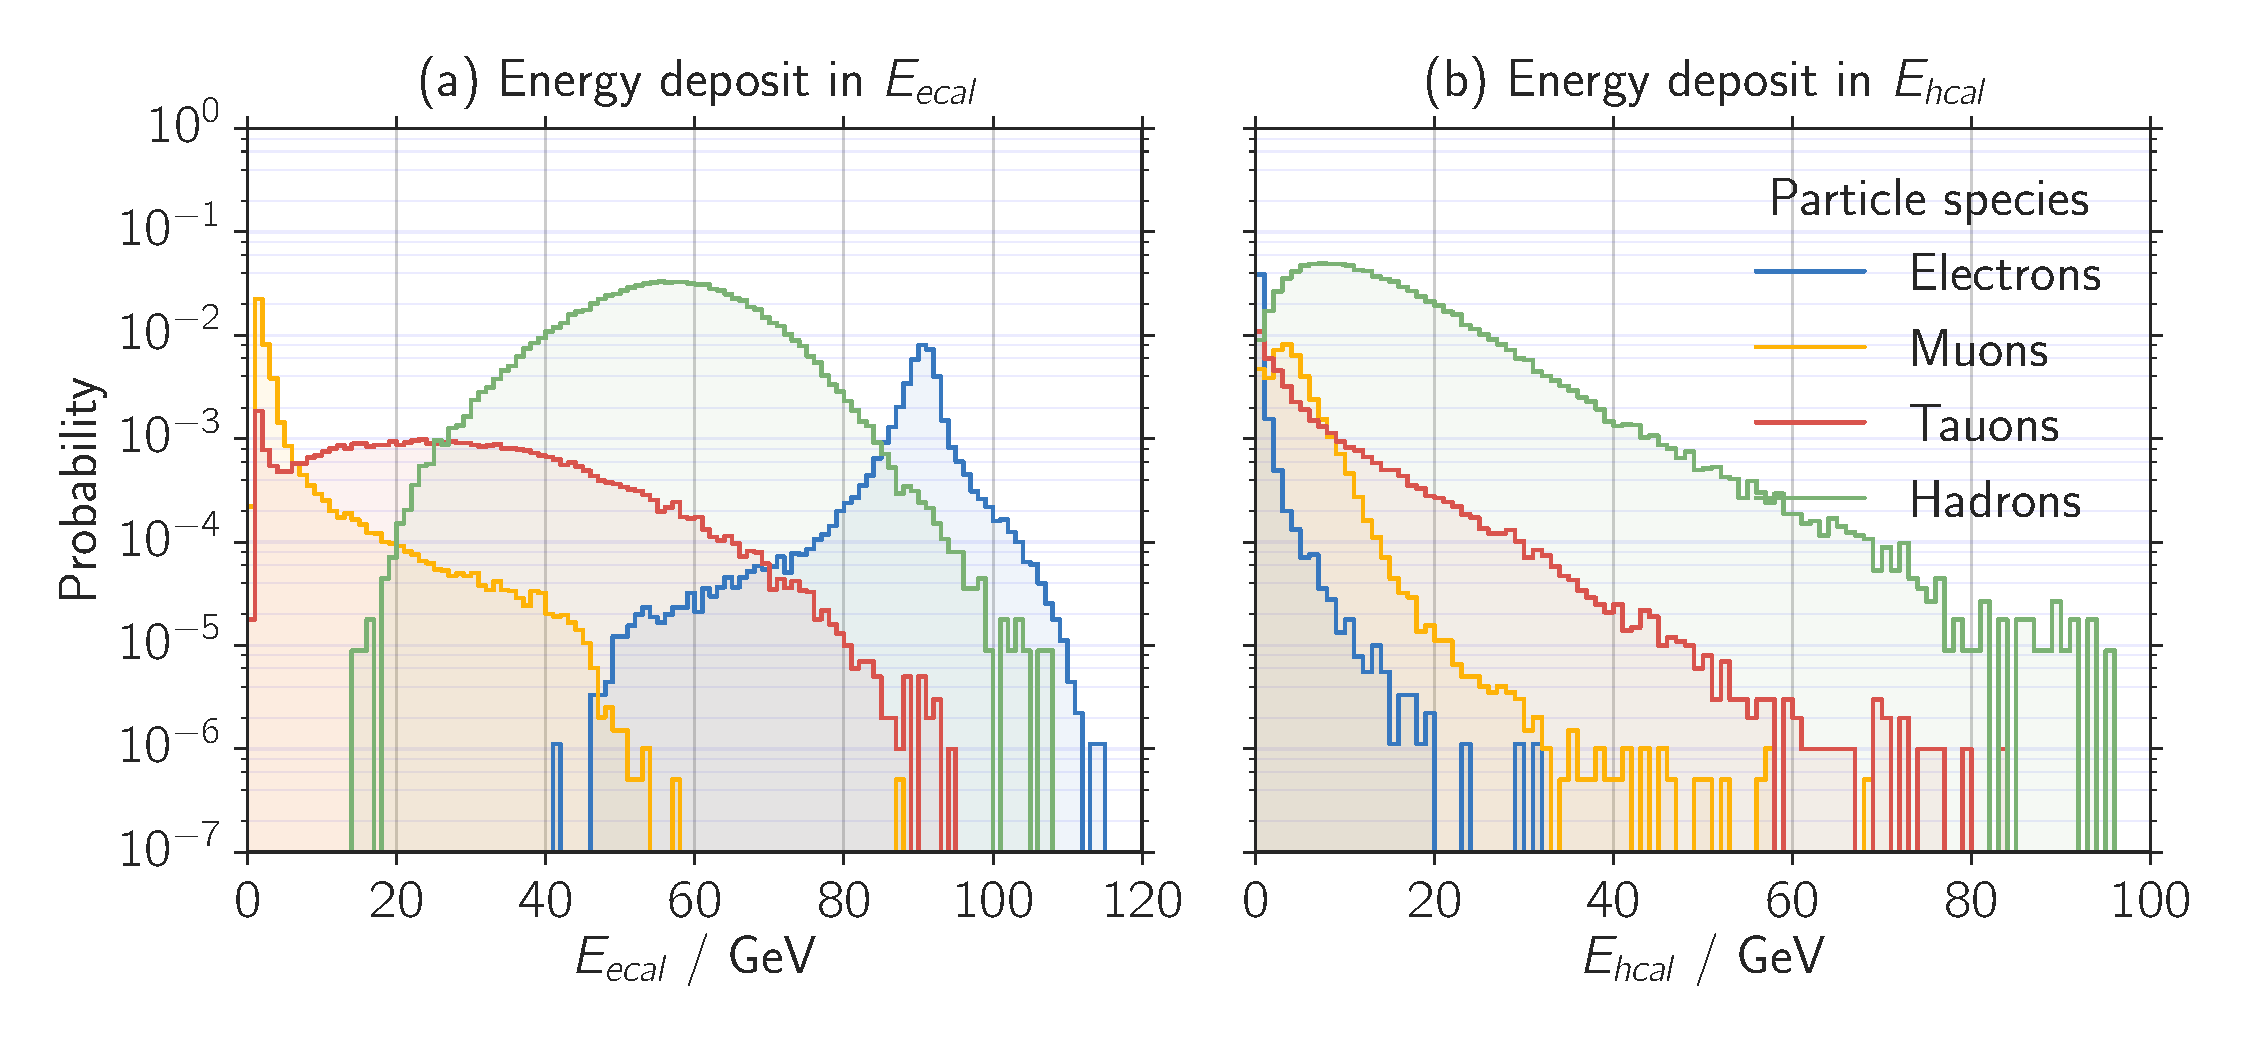
\includegraphics[width=1.0\linewidth]{figures/E_cal}
    \caption{bla}
\label{fig:monte1}
\end{figure}

\begin{figure}[htpb]
    \centering
    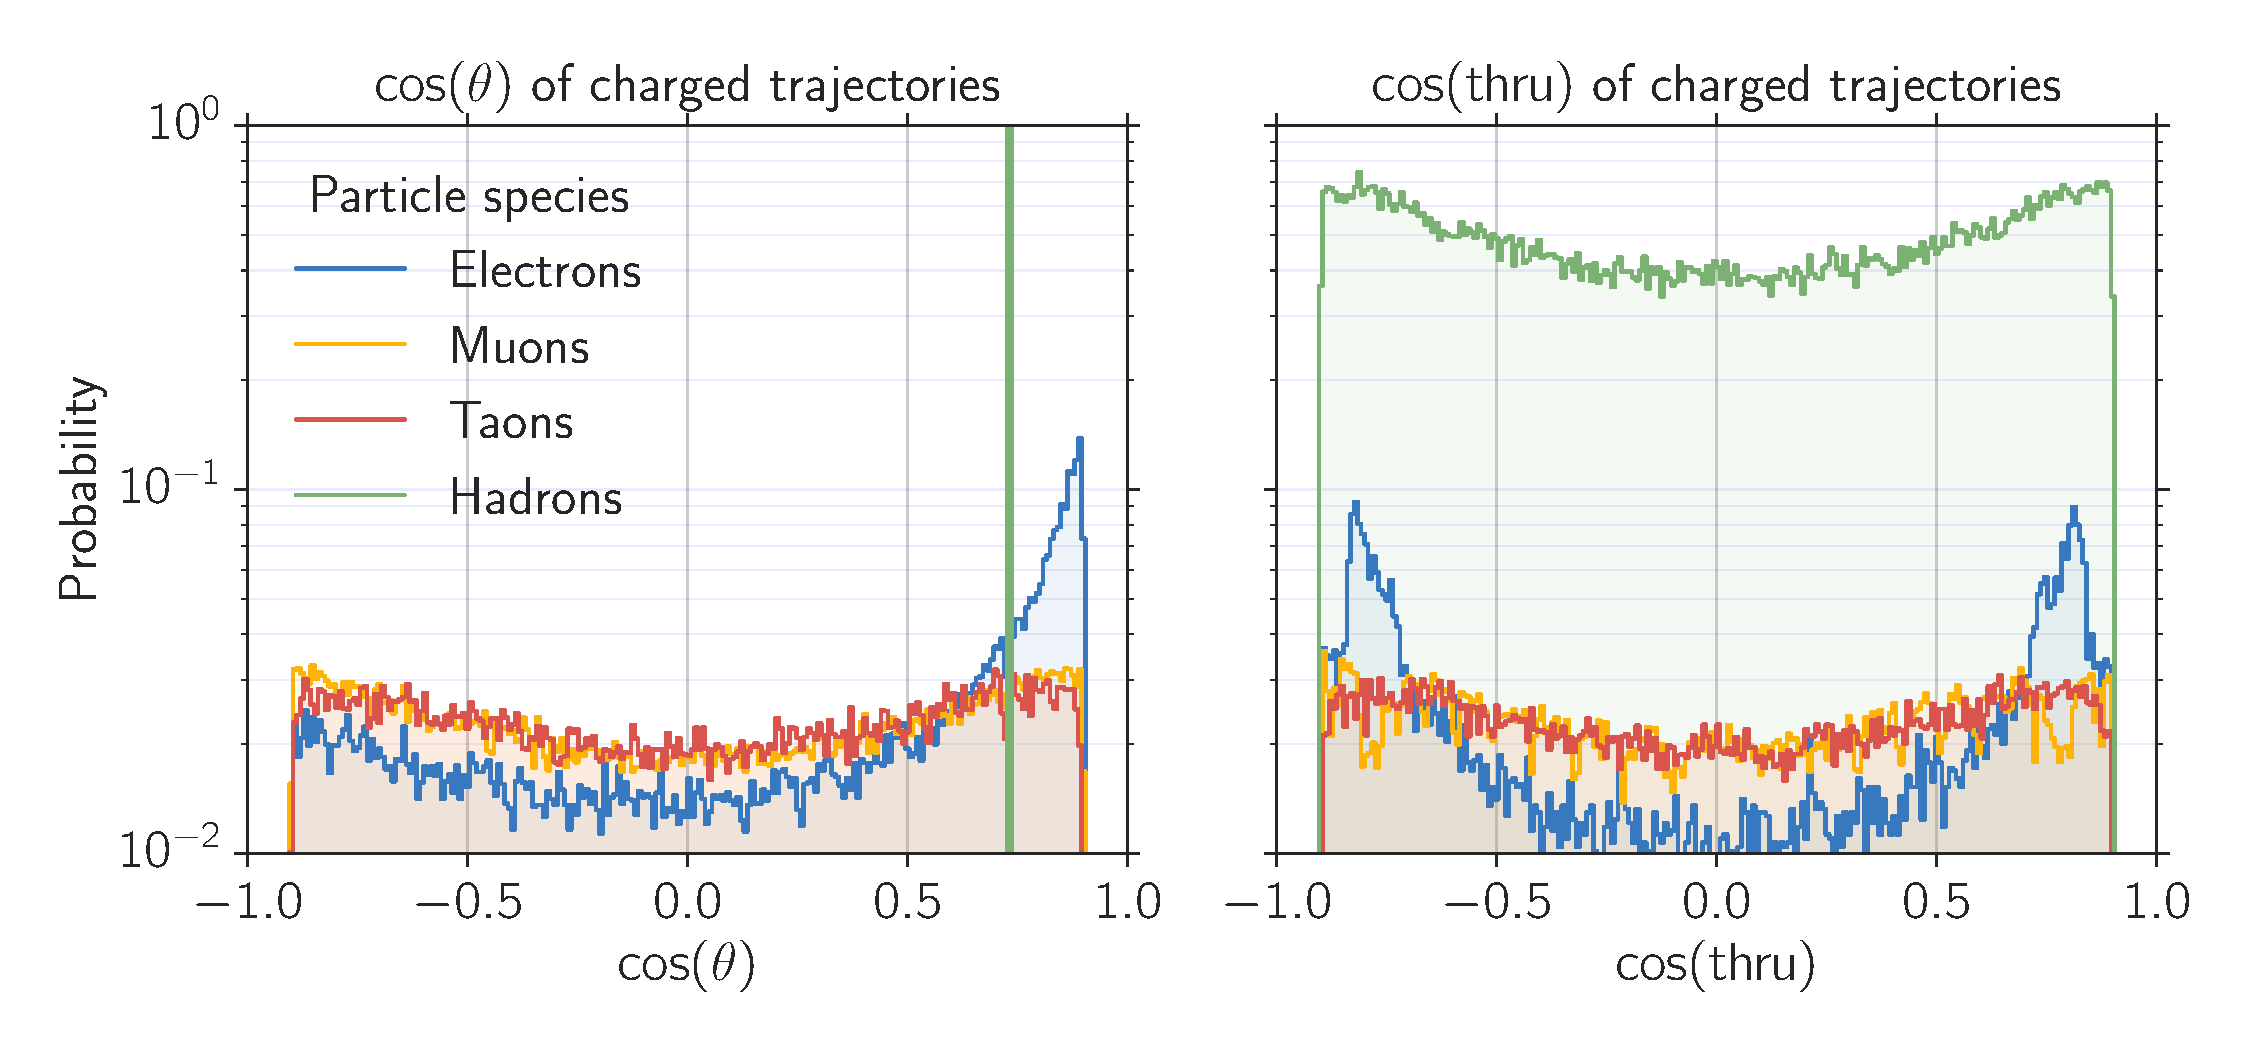
\includegraphics[width=1.0\linewidth]{figures/cos_figs}
    \caption{bla blupp}
    \label{fig:cos_figs}
\end{figure}
\subsubsection{Fitting Ts Channel}
\label{ssub:Fitting Ts Channel}

\begin{figure}[htpb]
    \centering
    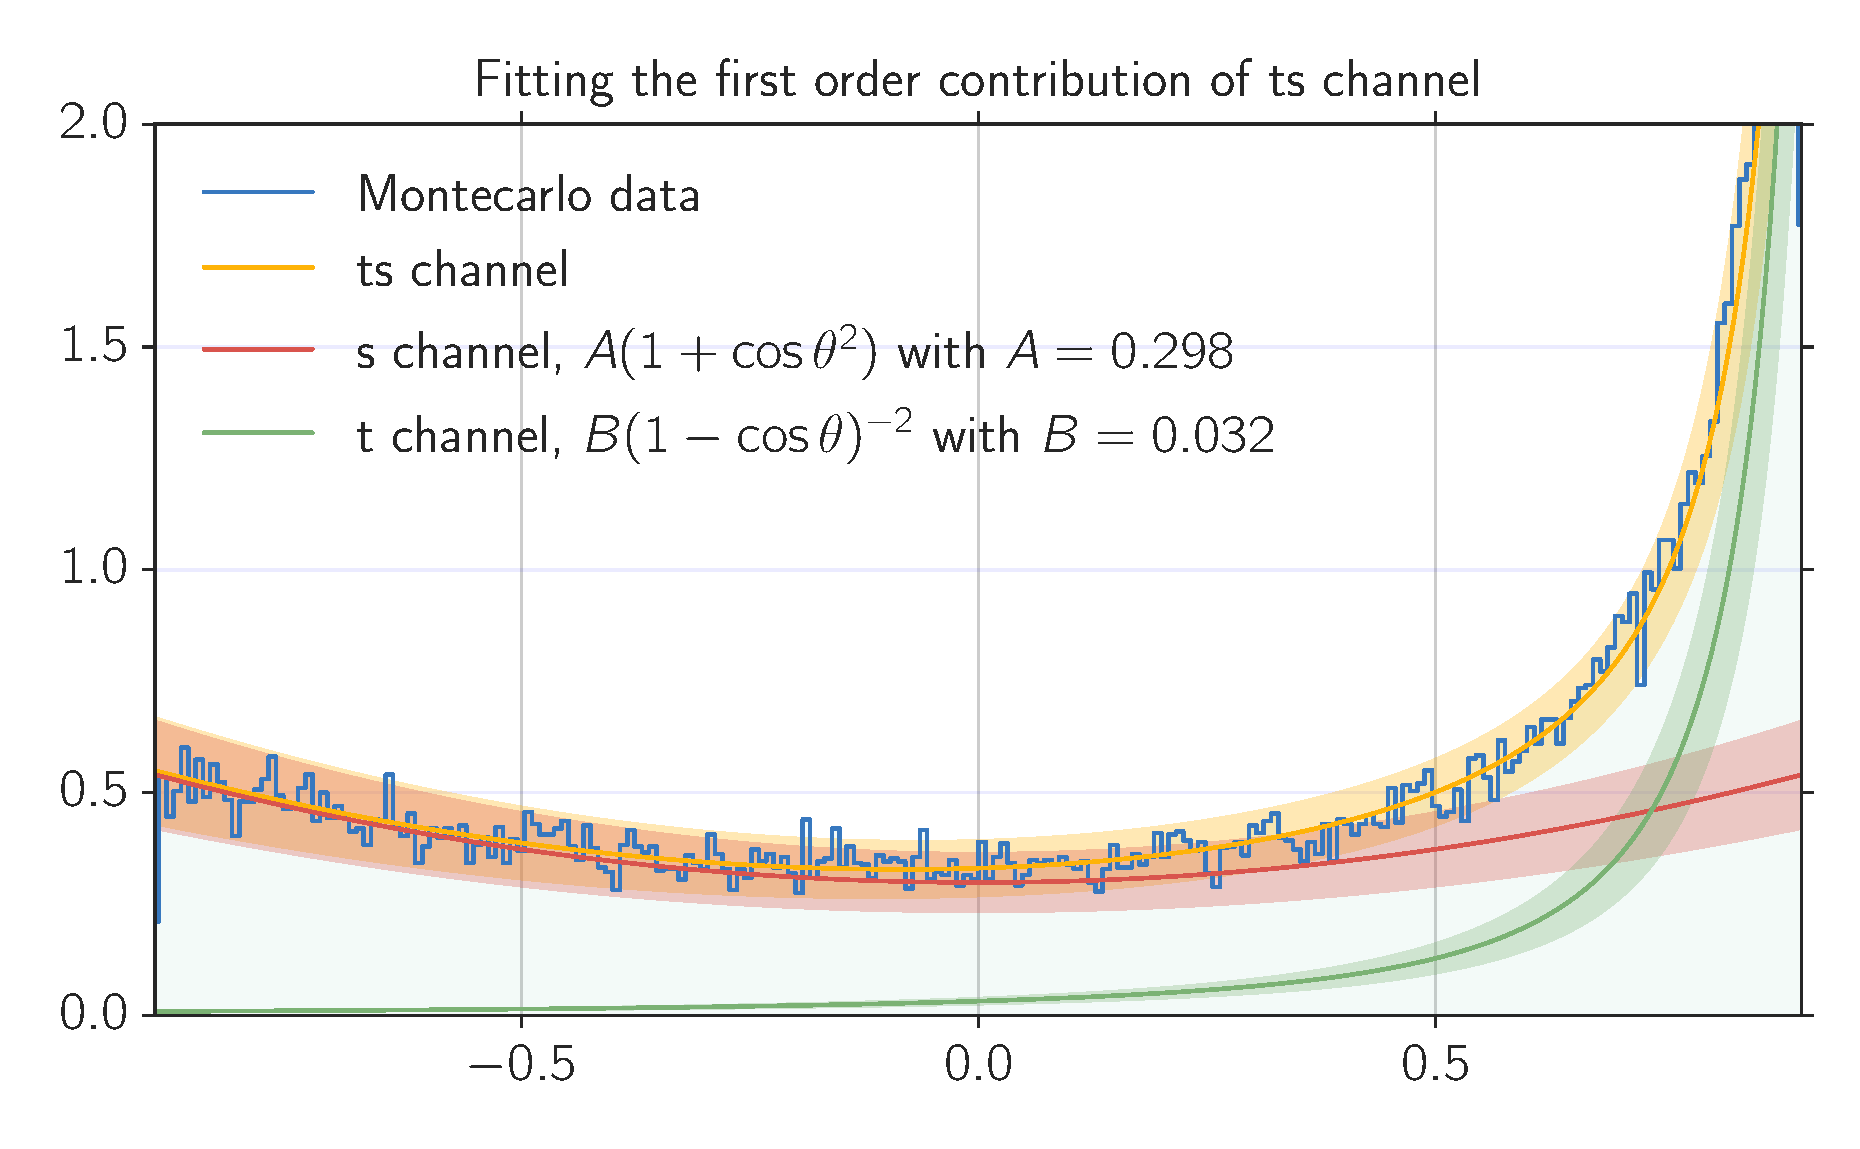
\includegraphics[width=1.0\linewidth]{figures/tschannel}
    \caption{bla blupp}
    \label{fig:tschannel}
\end{figure}

